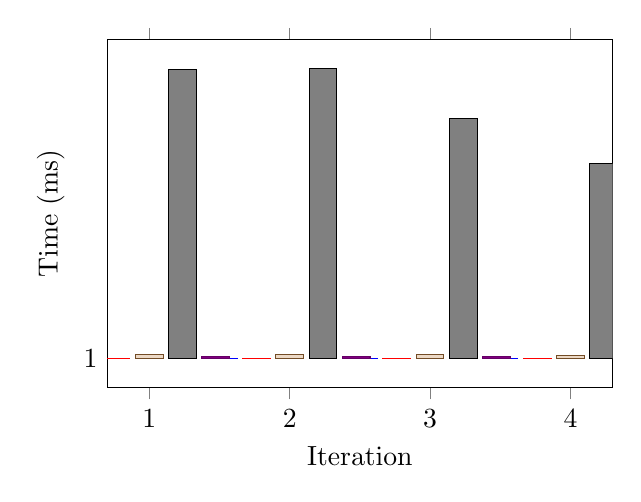
\begin{tikzpicture}
\begin{axis}[ybar, height=6cm, width=8cm, ytick=data, yticklabels={1, 64, 16K, 1M, Max}, xtick=data, xticklabels={1, 2, 3, 4}, xlabel=Iteration, ylabel=Time (ms), legend pos=north west, legend style={at={(0.5,1.03)}, anchor=north, draw=none}]
\addplot coordinates {(1, 0.16) (2, 0.16) (3, 0.16) (4, 0.16)};
\addplot coordinates {(1, 0.42) (2, 0.39) (3, 0.38) (4, 0.34)};
\addplot coordinates {(1, 67.86) (2, 68.10) (3, 56.50) (4, 45.91)};
\addplot coordinates {(1, 4333.76) (2, 4348.58) (3, 3607.68) (4, 2928.72)};
\addplot coordinates {(1, 29.54) (2, 29.43) (3, 35.48) (4, 43.71)};
\end{axis}
\end{tikzpicture}
